% !TeX spellcheck = en_US

\begin{frame}
	\Subsection{Linear Systems of Equations}
	~\\
		\underline{Aim:}\\
		\begin{center}
				\textit{	Given $A\in\mathbb{R}^{m\times n}$ ($m\neq n$ possible) and $b\in\mathbb{R}^m$,
				find $x\in\mathbb{R}^n$ such that\\
				$Ax=b.$}
		\end{center}
		~\\~\\
		\Subsubsection{Motivation: Curve Fitting}
		\Hide{
		As a motivating example let us consider \textit{curve fitting}.\\~\\
		Assume we are given $m\in\mathbb{N}$ measurements $(z_1,y_1),\dots,(z_m,y_m)\in\mathbb{R}^2$ (or more generally in any product space, say $Z\times Y$)\\ ~\\
		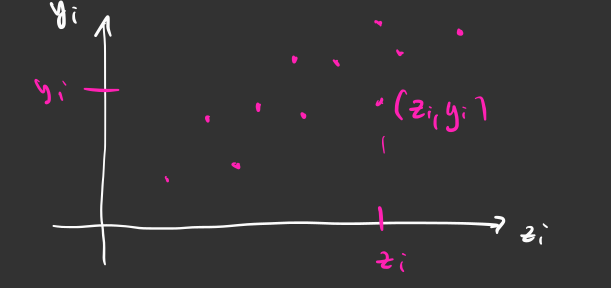
\includegraphics[width=0.5\linewidth]{curve-fitting}
	}
\end{frame}
\begin{frame}
\Hide{	\textbf{Question:}
	 Is there a ``significant'' relation between the $z_i$ and $y_i$?\\~\\
	 Let us consider the $z_i$ as input (independent/explanatory/exogenous) variable,\\
	 and the $y_i$ as output (dependent/predicted/response...) variable.\\~\\
	 {Examples: $z_i$ = (temperature, light intensity), $y_i$ = plant height or $z_i$ = year, $y_i$ = global mean temperature}\\
	 ~\\~\\
	 \textbf{Mathematically asking:} Is there a function $f$, so that
	 $
	 f(z_i)\cong y_i~\text{ for all $i=1,\ldots,m$?}
	 $
	 ~\\~\\~\\
	 \begin{minipage}[t]{0.48\textwidth}
	 		 \underline{Exact fit:} \textbf{Interpolation}\\
	 	$$f(z_i)=y_i~\forall i=1,\dots,m$$
	 	~\\
	 		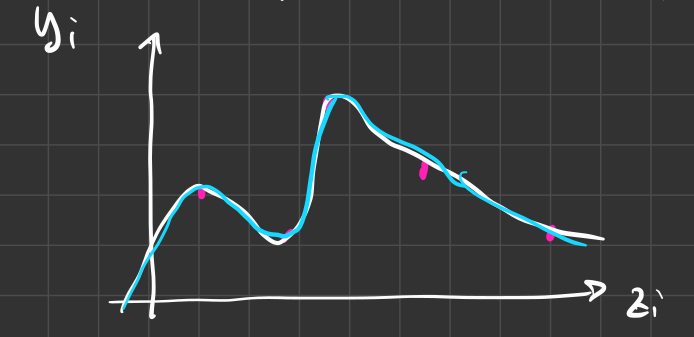
\includegraphics[width=0.7\linewidth]{interpolation-hand}
	 \end{minipage}
\begin{minipage}[t]{0.48\textwidth}
	 \underline{Approximate fit:} \textbf{Regression/Smoothing}\\
$$f(z_i)\approx y_i~\forall i=1,\dots,m$$
 ~\\
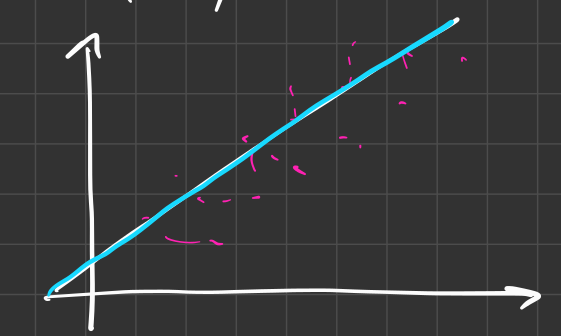
\includegraphics[width=0.7\linewidth]{regression-hand}
\end{minipage}
}
\end{frame}
\begin{frame}
	~\\
	\Hide{
		In order to find such a fit, we need to restrict ourselves to certain classes of functions $f$. With other words we need to assume a certain ''model'':\\
		$$z_i\stackrel{f}{\mapsto}y_i$$\\
		~\\
		In this course we will consider models of the following kind:
		$$
		f:\mathbb{R}\rightarrow\mathbb{R},~~f(z):=\sum_{k=1}^{n}x_kf_k(z)
		$$
\begin{itemize}
	\item[$\rightarrow$] More precisely, we assume that the relation between the $z_i$ and the $y_i$ can be modeled by a \textit{linear combination}		 of $\underbrace{\text{some functions}~f_k:\mathbb{R}\rightarrow\mathbb{R}}_{\textit{\color{header}given by assumption}}$ 
		with 
		$\underbrace{\text{some coefficients/parameters}~x_k}_{\color{header}\textit{to be determined}~(f(z_i)\cong y_i)}$
		\item [] {\small (More generally $f,f_k\colon \R^k \to \R$. Important here is the fact that our model $f$ is linear combined from the $f_k$.)}
\end{itemize}
		~\\
\begin{example}[Polynomial Interpolation/Regression]
	One often considers a polynomial model:
		$$
		 f_k(z) := z^{k-1},~~\text{so that}~~f(z)=x_1+x_2z+x_3z^2+\dots+x_nz^{n-1}
		$$
		For example, if $n=2$ then $f(z)=x_1+x_2z$ (an affine linear model).
\end{example}
	}
\end{frame}

\begin{frame}
	~\\
	\Hide{
		\textbf{How does this translate into a linear system ``$Ax \cong b$''?}\\
		~\\
		For all measurements $(z_1,y_1),\dots,(z_m,y_m)$ we require:
		$$
		\sum_{k=1}^{n}x_kf_k(z_i)=f(z_i)\cong y_i~~\text{for all}~i=1,\dots,m
		$$
		Writing these equations row by row for each $i$-th measurement gives:
		\begin{align*}
&\begin{matrix}
i=1:&x_1f_1(z_1)+x_2f_2(z_2)+\dots+x_nf_n(z_1)&=y_1\\
\vdots&\vdots&\vdots\\
i=m:&x_1f_1(z_m)+x_2f_2(z_m)+\dots+x_nf_n(z_m)&=y_m
\end{matrix}
\end{align*}
Using matrix notation, this system can be written as:
$$
\underbrace{
	\begin{pmatrix}
	f_1(z_1)&\cdots&f_n(z_1)\\
	\vdots&\ddots&\vdots\\
	f_1(z_m)&\cdots&f_n(z_m)
	\end{pmatrix}}_{=:A\in\mathbb{R}^{m\times n}}
\underbrace{\begin{pmatrix}x_1\\x_2\\\vdots\\x_n\end{pmatrix}}_{=:x\in\mathbb{R}^n}
\cong\underbrace{\begin{pmatrix}y_1\\\vdots\\y_m\end{pmatrix}}_{=:b\in\mathbb{R}^m} 
~~~\Leftrightarrow~~~
Ax\cong b
$$
~\\
$\rightarrow$ Also revisit Example \ref{ex:interpolation}.
	}
\end{frame}

\begin{frame}
	~\\
	\Hide{
		\begin{minipage}[t]{0.48\textwidth}
			\underline{Exact:} \textbf{Interpolation}
		$$
		Ax=b
		$$
		\end{minipage}
%%
	\begin{minipage}[t]{0.48\textwidth}
		\underline{Approximate:} \textbf{Regression}
$$
Ax\approx b
$$
A common approach to address a regression problem is a linear least squares formulation:
\begin{align*}
\min_{x\in\mathbb{R}^n}~\|Ax-b\|_2^2 ~&=~\sum_{i=1}^m(Ax-b)_i^2\\
&=~\sum_{i=1}^m(f(z_i)-y_i)^2
\end{align*}
~\\
	\begin{figure}
		\centering
		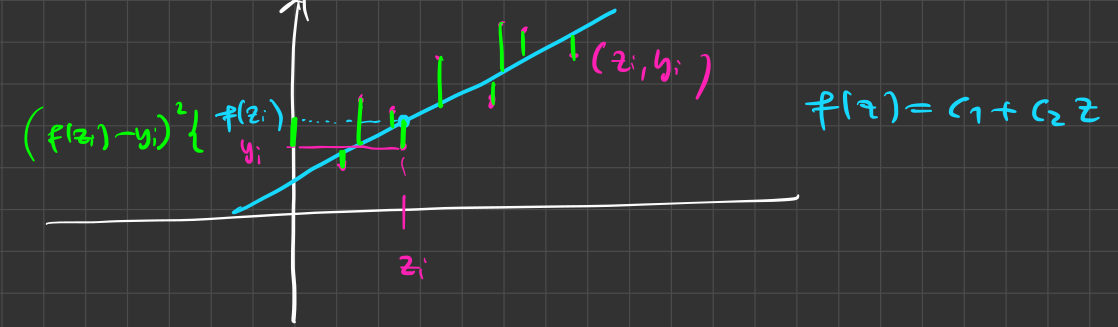
\includegraphics[width=1.1\linewidth]{regression-linear}
		\end{figure}

	\end{minipage}


	}
\end{frame}

\begin{frame}
	\Subsubsection{Existence and Uniqueness Analysis}
	\Hide{
		Let us consider the following cases:\\
\begin{figure}
	\centering
	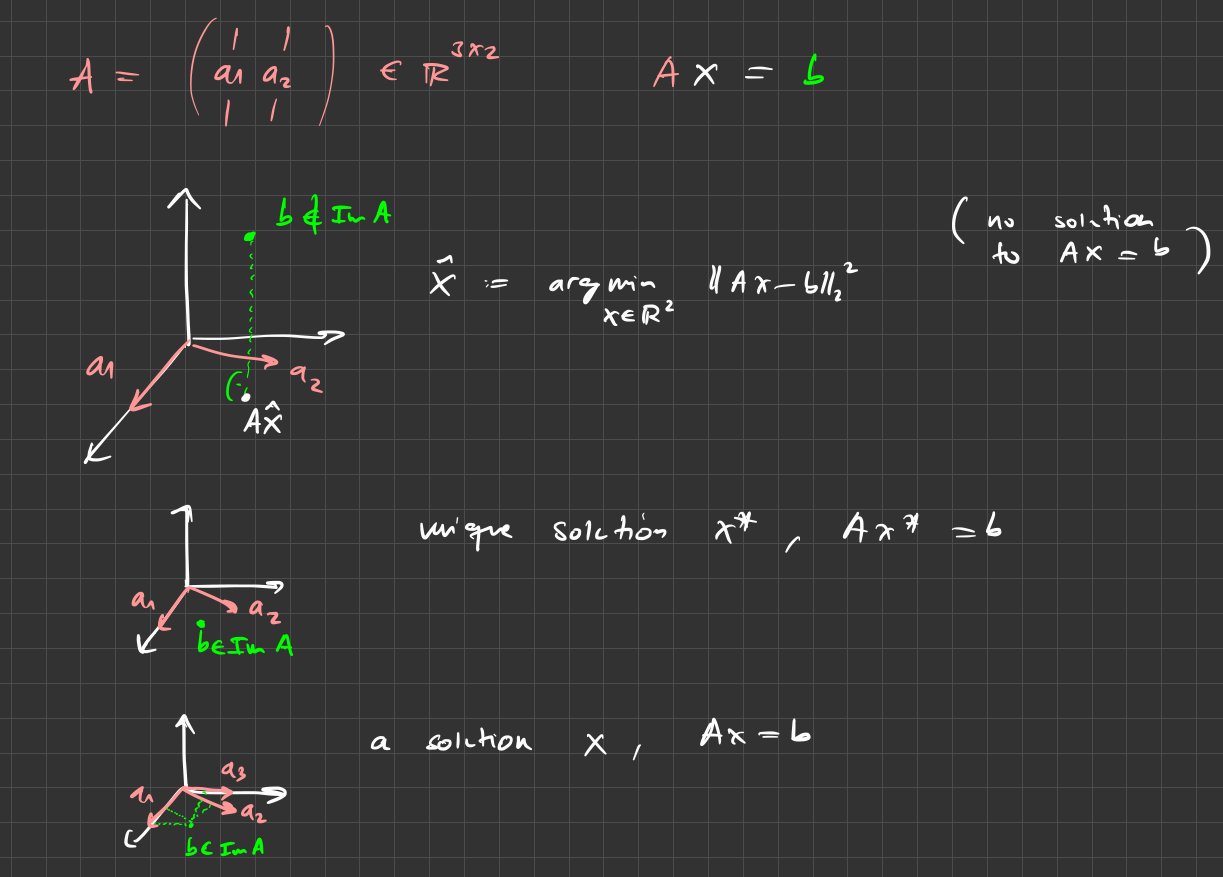
\includegraphics[width=0.85\linewidth]{existence-uniqueness-linsys}
%	\caption{}
%	\label{fig:existence-uniqueness-linsys}
\end{figure}



	}
\end{frame}
\begin{frame}
\textit{Summary}\\~\\
	\textbf{Aim:} \vspace*{-0.5cm}
\begin{center}
	\textit{Given $A\in\mathbb{R}^{m\times n}$ ($m\neq n$ possible) and $b\in\mathbb{R}^m$,
		find $x\in\mathbb{R}^n$ such that\\
		$Ax=b.$}
\end{center}
\Hide{Here:
\begin{itemize}
	\item[$m$]$=~\sharp$ equations $=~\sharp$ measurements $=$ length of the column vectors\\
	\item[$n$]$=~\sharp$ unknowns $=~\sharp$ parameters $=~\sharp$ columns\\
\end{itemize}
	~~~~~~$\begin{matrix}~&{\color{cyan}n}\\A=~{\color{cyan}m}&\begin{pmatrix}|&~&|\\a_1&\cdots&a_n\\|&~&|\end{pmatrix}\end{matrix}$,~~~with image Im$(A)=\{Ax:\in\mathbb{R}^n\}~=$ span$(a_1,\dots,a_n)$\\
	~\\~\\
	Let us define the solution set
	$$S:=\{x\in\mathbb{R}^n:Ax=b\}~=~f_A^{-1}(\{b\}),$$
	then there are three possible states, namely,
	$$
	|S|=~\begin{cases}
	 	&0~:~\text{``no solution'', if~~}b\notin\text{Im}(A)\\
	 &1~:~\text{``unique solution'', if~~}b\in\text{Im}(A)~\text{and independent columns}~(\text{ker}(A)=\{0\})\\
	 &\infty~:~\text{``infinitely many solutions'', if~~}b\in\text{Im}(A)~\text{and dependent columns}~(\text{ker}(A)\neq\{0\})
	\end{cases}
	$$
	For a given $b$, observe the relations between image and existence as well as kernel and uniqueness. In fact,
	$b\in$ or $\notin\text{Im}(A)$ decides if solutions \textbf{exist} and \text{ker}(A) $=$ or $\neq~\{0\}$ gives the solutions' \textbf{uniqueness}.}
\end{frame}
%
%
\begin{frame}
	\Hide{
	Quick clarification:\\~\\
	Let $\ker(A)\neq \{0\}$, then there exists a $w \in \Rn$ so that $$A (\alpha w)= 0$$ for \textit{all} scalars $\alpha \in \R $.\\~\\
	If $b\in\im(A)$, then there exists an $x \in \Rn$, so that $$Ax = b.$$
	Adding these two equations gives
	$$A(x + \alpha w) = b ~~~\forall \alpha \in \R .$$ 
	With other words, we find infinitely many solutions.\\~\\
	Another equivalent argument in view of Lemma \ref{lem:linear-independence}: A nontrivial kernel implies that the columns are linearly dependent and thus vectors in their span are not uniquely combined. Now we see that this already implies infinitely many ways to linearly combine the columns of $A$ to obtain $b$ (assumed $b$ lies in there span).
}
\end{frame}